\documentclass{article}
\usepackage{graphicx}
\usepackage{caption}
\usepackage{subcaption}
\usepackage{booktabs}
\usepackage{multirow}
\usepackage{tabularx}
\usepackage{adjustbox}
\usepackage{amssymb}
\usepackage{xcolor}
\usepackage{hyperref}
\definecolor{AdviseTeal}{HTML}{1F7A7A}
\newenvironment{ack}{\section*{Acknowledgments}}{}
\newcommand{\aff}[1]{\textsuperscript{#1}}
\newcommand{\leadmark}{\textsuperscript{\(\star\)}}
\def\equalcontrib{\textsuperscript{\(\dagger\)}}
\newcommand{\advisemark}{\textsuperscript{\(\ddagger\)}}

\title{Seeing the Whole Room: Panoramic Reasoning for Multimodal Models}
\author{%
  Jiawei Gu\aff{1}\leadmark \quad Linjie Li\aff{1}\leadmark \quad Yiming Liu\aff{2}\equalcontrib \quad Yunzhuo Hao\aff{3}\equalcontrib \quad Huichen Wang\aff{1}\equalcontrib \\
  \bfseries Guanzheng Chen\aff{4}\equalcontrib \quad Zhichao Peng\aff{5} \quad  Luxin Xu\aff{6} \quad Xinyu Zhang\aff{6} \quad Li Luo\aff{7} \\
  \bfseries Disen Lan\aff{6} \quad Zican Hu\aff{8} \quad Mingyang Song\aff{6} \quad David Valente\aff{4} \quad Alex Jinpeng Wang\aff{5} \\
  \bfseries Yafu Li\aff{9} \quad Ganqu Cui\aff{2} \quad Zhengyuan Yang\aff{10} \quad Qizhe Xie\aff{4}\advisemark \\
  \bfseries Yejin Choi\aff{11}\advisemark \quad Ranjay Krishna\aff{1}\advisemark \quad Yu Cheng\aff{9}\advisemark \\[6pt]
  \normalfont\small
  \aff{1}University of Washington \quad \aff{2}Tsinghua University \quad \aff{3}Zhejiang University \\
  \normalfont\small \aff{4}National University of Singapore \quad \aff{5}Central South University \quad \aff{6}Fudan University \\
  \normalfont\small \aff{7}The University of Hong Kong \quad \aff{8}Nanjing University \quad \aff{9}The Chinese University of Hong Kong \\
  \normalfont\small \aff{10}University of Rochester \quad \aff{11}Stanford University \\[4pt]
  \normalfont\small
  \leadmark\,Project lead \qquad \equalcontrib\,Equal contribution \qquad \advisemark\,Equal advising
}
\date{}

\begin{document}
\maketitle
\vspace{-18pt}
{\centering\small\hypersetup{urlcolor=AdviseTeal}
  \url{https://thinkmorph.github.io/ssl/}\par
}
\vspace{4pt}

\begin{abstract}
We study panoramic reasoning in multimodal models.

\end{abstract}

\section{Introduction}
Models see the whole room.


\section{Results}
Figure~\ref{fig:case-failure} and Figure~\ref{fig:cost} sit side by side.

\begin{figure}[ht]
\centering
\captionsetup{position=bottom,belowskip=0pt}
\begin{minipage}[t]{0.49\linewidth}
\centering
\parbox[c][0.65\linewidth][c]{\linewidth}{\centering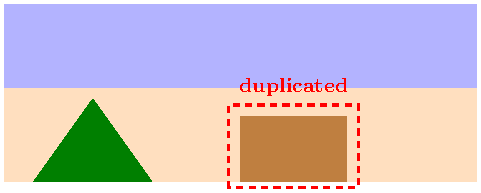
\includegraphics[width=\linewidth]{figures/case_failure_mmsi.pdf}}
\caption{\textbf{A low-fidelity panorama leads to an error.} Key objects are missing or duplicated.}
\label{fig:case-failure}
\end{minipage}\hfill
\begin{minipage}[t]{0.49\linewidth}
\centering
\parbox[c][0.65\linewidth][c]{\linewidth}{\centering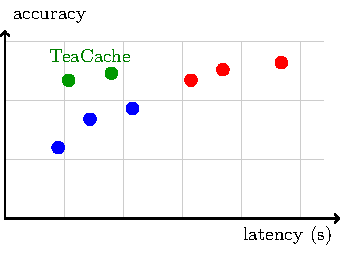
\includegraphics[width=\linewidth]{figures/cost_scatter.pdf}}
\caption{\textbf{Accuracy and latency on V$^\star$.} TeaCache reduces latency without lowering accuracy.}
\label{fig:cost}
\end{minipage}
\end{figure}

A plain figure follows.

\begin{figure}[t]
  \centering
  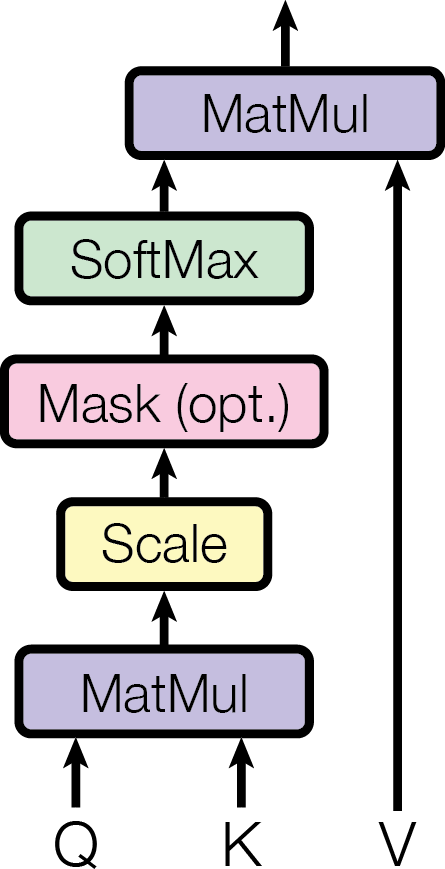
\includegraphics[width=0.6\linewidth]{figures/attention.png}
  \caption{Scaled dot-product attention.}
  \label{fig:plain}
\end{figure}

\begin{figure*}[t]
  \centering
  \begin{subfigure}[b]{0.48\textwidth}
    \centering
    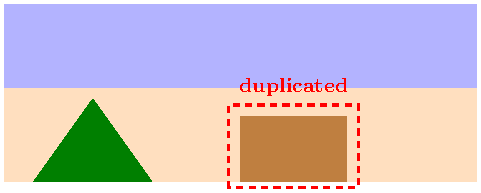
\includegraphics[width=\textwidth]{figures/case_failure_mmsi}
    \caption{Panorama}
    \label{fig:sub-a}
  \end{subfigure}
  \hfill
  \begin{subfigure}[b]{0.48\textwidth}
    \centering
    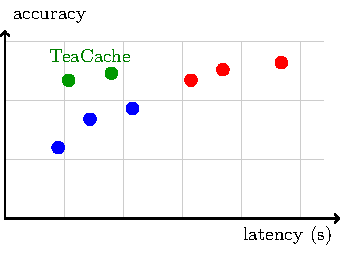
\includegraphics[width=\textwidth]{figures/cost_scatter.pdf}
    \caption{Cost}
    \label{fig:sub-b}
  \end{subfigure}
  \caption{Two subfigures with their own captions.}
  \label{fig:subs}
\end{figure*}

\section{Tables}

\begin{table}[t]
  \centering
  \caption{Main results. Best in \textbf{bold}.}
  \label{tab:main}
  \begin{tabular}{lccc}
    \toprule
    Method & Acc.\ (\%) & Latency (s) & $\Delta$ \\
    \midrule
    Baseline & 61.2 & 4.10 & -- \\
    TeaCache & \textbf{64.8} & \textbf{2.35} & +3.6 \\
    \bottomrule
  \end{tabular}
\end{table}

\begin{table*}[t]
  \centering
  \caption{Per-category accuracy with grouped headers.}
  \label{tab:wide}
  \resizebox{\textwidth}{!}{%
  \begin{tabular}{l|cc|cc}
    \toprule
    \multirow{2}{*}{Model} & \multicolumn{2}{c|}{Indoor} & \multicolumn{2}{c}{Outdoor} \\
    \cmidrule(lr){2-3}\cmidrule(lr){4-5}
     & Count & Relation & Count & Relation \\
    \midrule
    GPT-4o & 52.1 & 48.0 & 55.3 & 50.2 \\
    Ours & 60.4 & 57.9 & 61.0 & 58.8 \\
    \bottomrule
  \end{tabular}}
\end{table*}

\begin{table}[t]
  \centering
  \caption{A tabularx and a tabular* in adjustbox.}
  \label{tab:x}
  \begin{tabularx}{\linewidth}{lX}
    \toprule
    Term & Meaning \\
    \midrule
    MMSI & Multi-modal spatial intelligence, a benchmark of questions about rooms. \\
    \bottomrule
  \end{tabularx}
  \vspace{4pt}
  \begin{adjustbox}{max width=\linewidth}
  \begin{tabular*}{\linewidth}{@{\extracolsep{\fill}}lrr}
    \hline
    Split & Questions & Images \\ \hline
    Train & 12{,}000 & 3{,}400 \\
    Test & 1{,}000 & 300 \\ \hline
  \end{tabular*}
  \end{adjustbox}
\end{table}

\begin{ack}
This project was partially funded by Samsung and by SRC CoCoSys.
\end{ack}

\bibliographystyle{plain}
\bibliography{main}

\appendix
\raggedbottom
\section{Extra results}
More tables.


\newpage
\section*{Checklist}
All claims hold.


\end{document}
